\chapter[Gerenciamento de requisitos]{Gerenciamento de requisitos}
O tratamento de requisotos na metodologia ágil é fundamentalmente diferente. Isso pode ser imediatamente observado nos princípios ágeis:
\begin{enumerate}
\item A nossa maior prioridade é satisfazer o cliente através de entregas adiantadas e contínuas de software com valor agregado.
\item Abraçar às mudanças nos requisitos, mesmo em estágios avançados do desenvolvimento. O processo ágil encoraja as mudanças visando vantagens competitivas para o ciente.
\end{enumerate}

Com o ágil, nós temos uma abordagem muito mais flexível para o gerenciamento de requisitos: uma temporária, interativa e pontual. As especificações de requisitos tradicionais não cabem aqui, assim como as de design. E juntamente com isso, temos o comprometimento de entregar "tudo" em um calendário fixo e uma base de recursos fixos~\cite{leffingwell}.
\section{Atributos de um requisito}
Os atributos contém as informações mais importantes daquele requisito, são suas propriedades, e é a partir dessas propriedades que se tem informações como: data de criação, origem, importância, dentre outras. Demandam atenção durante a sua especificação, pois fornecem importantes informações sobre o estado do projeto, além de permitirem que sejam realizadas consultas dentro de todos os requisitos.
Os atributos definidos para gerenciar os requisitos durante a execução do nosso projeto foram:
  \begin{figure}[!htbp]
    \centering
    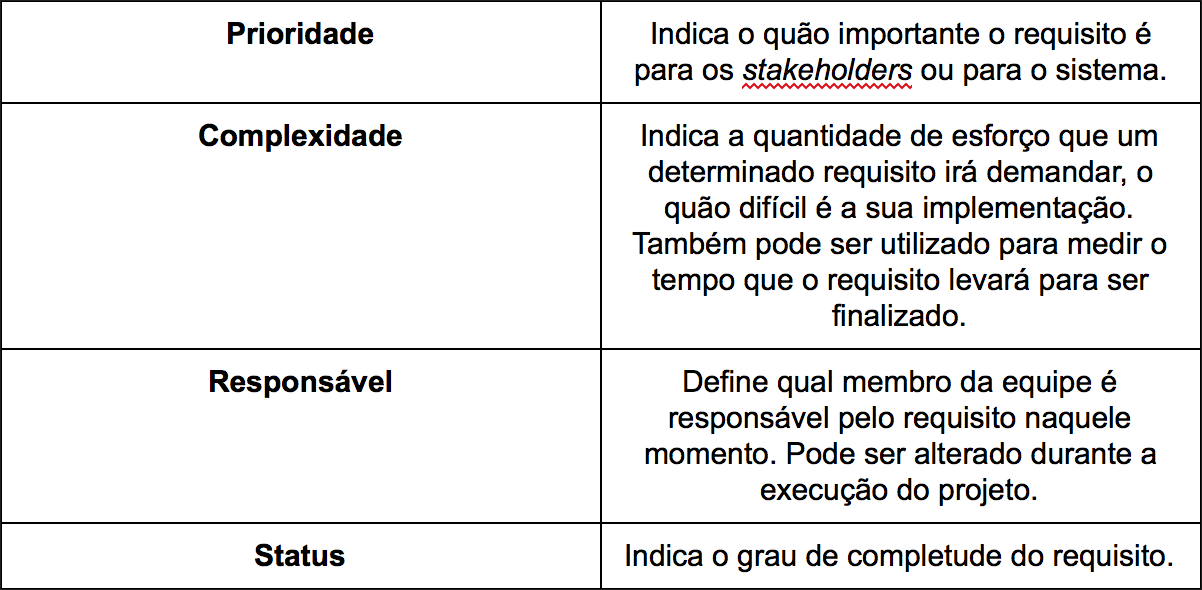
\includegraphics[scale=0.65]{figuras/tabela_atributos}
    \caption[Atributos dos requisitos do projeto]{Atributos dos requisitos do projeto. \footnotemark}
    \label{tabela_atributos}
  \end{figure}
  
  Exemplo de matriz de atributos de requisitos:
    \begin{figure}[!htbp]
    \centering
    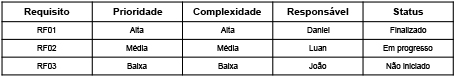
\includegraphics[scale=0.65]{figuras/matriz_atributos}
    \caption[Matriz de atributos do projeto.]{Matriz de atributos do projeto. \footnotemark}
    \label{tabela_matriz_atributos}
  \end{figure}
\subsection{Prioridade}
  \begin{figure}[!htbp]
    \centering
    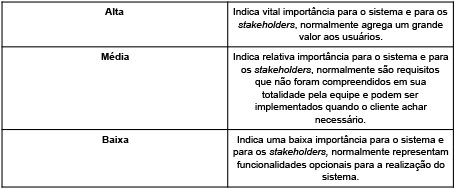
\includegraphics[scale=0.5]{figuras/tabela_prioridade}
    \caption[Prioridade dos requisitos do projeto.]{Prioridade dos requisitos do projeto. \footnotemark}
    \label{tabela_prioridade}
  \end{figure}
\subsection{Complexidade}
  \begin{figure}[!htbp]
    \centering
    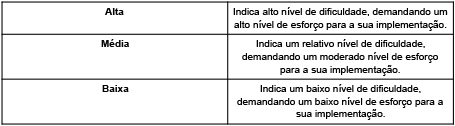
\includegraphics[scale=0.5]{figuras/tabela_complexidade}
    \caption[Complexidade dos requisitos do projeto.]{Complexidade dos requisitos do projeto. \footnotemark}
    \label{tabela_complexidade}
  \end{figure}
\subsection{Responsável}
Identifica na equipe o membro responsável pelo requisito naquele momento.
\subsection{Status}
  \begin{figure}[!htbp]
    \centering
    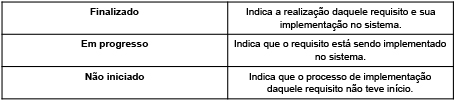
\includegraphics[scale=0.5]{figuras/tabela_status}
    \caption[Status dos requisitos do projeto.]{Status dos requisitos do projeto. \footnotemark}
    \label{tabela_status}
  \end{figure}
\section{Rastreabilidade de requisitos}
Rastreabilidade de software é a habilidade de relacionar artefatos criados durante o ciclo de vida de desenvolvimento de um sistema de software. Os elementos rastreáveis do projeto são chamados de itens de rastreabilidade.

As necessidades de rastreabilidade das diferentes partes interessadas, como: patrocinadores, gerentes, analistas, designers, mantenedores e usuários, diferem devido a mudanças em seus objetivos e prioridades. A rastreabilidade de requisitos é uma característica do sistema em que os requisitos estão claramente ligados às suas fontes, e os artefatos criados durante o ciclo de vida do desenvolvimento de sistemas com base nesses requisitos.

O rastreamento de requisitos pode ser visto como uma habilidade de acompanhar e descrever a vida de um requisito em abas as direções. A pré-rastreabilidade documenta o contexto a partir do qual emergem os requisitos, já a pós-rastreabilidade vincula os requisitos ao desenho do sistema e sua implementação~\cite{davis}.

\subsection{Classificações da rastreabilidade de requisitos}
A princípio, a rastreabilidade de requisitos consiste em duas propriedades, propriedades essas que embasam todo o rastreamento de requisitos.

A capacidade de rastrear um requisito até os seus refinamentos é definida como rastrear para frente(forwards), e a de rastrear um refinamento até sua origem é definida como rastrear para trás(backwards)~\cite{davis}. Deve-se atentar para ambas propriedades durante o processo de rastreabilidade, a fim de evitar falhas no mesmo. É imprescindível que seja mantida uma rastreabilidade bidirecional entre os requisitos.
No que diz respeito a rastreabilidade, existem dois ramos gerais, o de rastreabilidade horizontal e vertical e o de pré e pós-rastreabilidade.

  \begin{figure}[!htbp]
    \centering
    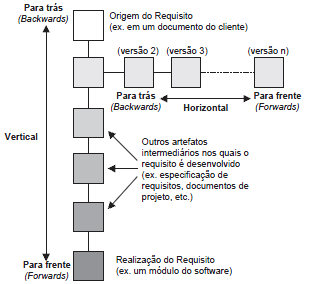
\includegraphics[scale=0.75]{figuras/tipos_de_rastreabilidade}
    \caption[Rastreabilidade horizontal e vertical.]{Rastreabilidade horizontal e vertical. \footnotemark}
    \label{ramos_rastreabilidade}
  \end{figure}
  \footnotetext{Fonte: \cite{tese_doutorado}}

\textbf{Rastreabilidade horizontal} - É a rastreabilidade entre diferentes versões ou variações de requisitos, ou outros artefatos, em particular uma fase do ciclo de vida\cite{tese_doutorado}.

\textbf{Rastreabilidade vertical} - É a rastreabilidade realizada entre requisitos e artefatos produzidos pelo processo de desenvolvimento ao longo do ciclo de vida do projeto.\cite{tese_doutorado}

  \begin{figure}[!htbp]
    \centering
    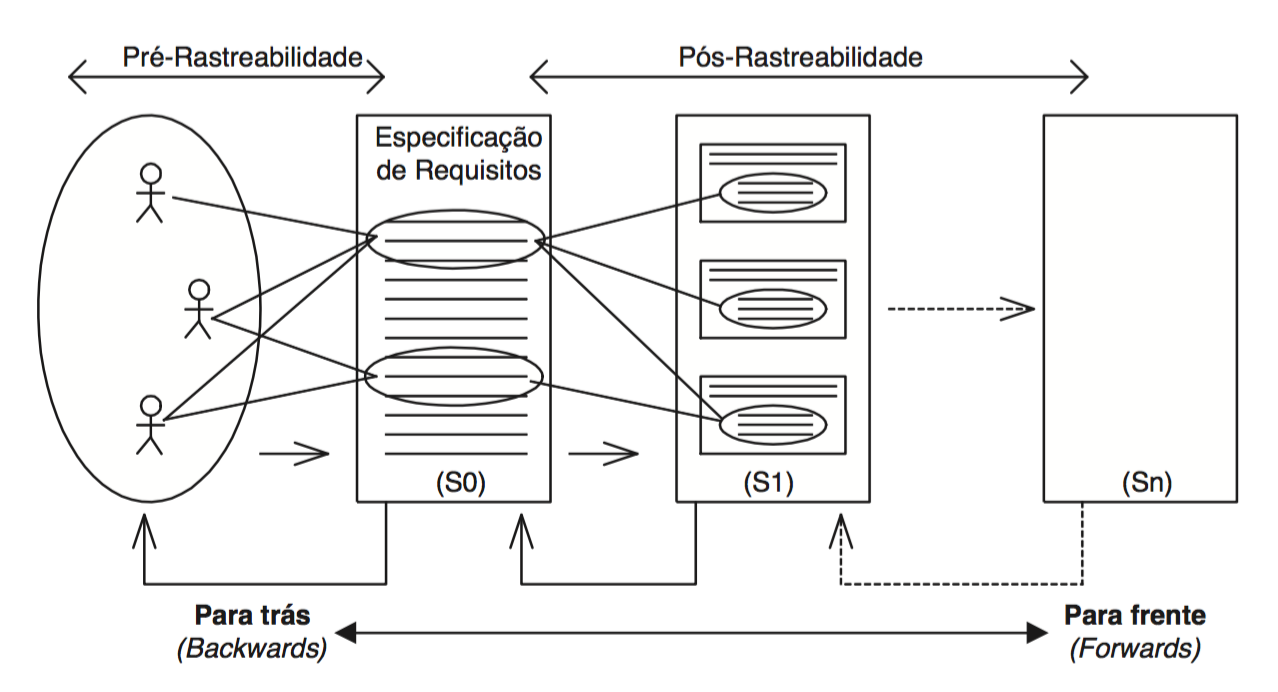
\includegraphics[scale=0.4]{figuras/pre_pos_rastreabilidade}
    \caption[Pré e pós-rastreabilidade.]{Pré e pós-rastreabilidade. \footnotemark}
    \label{pre_pos_rastreabilidade}
  \end{figure}
  \footnotetext{Fonte: \cite{tese_doutorado}}

\textbf{Pré-rastreabilidade} - Depende da capacidade da equipe em rastrear os requisitos para frente(\textit{forward}) e para trás(\textit{backwards}), partindo dos seus padrões e/ou fontes(clientes, usuários, normas e etc.) originais. Isso é feito analisando os artefatos gerados pelo processo de engenharia de requistos(requisitos funcionais, não-funcionais, validações, documentos de análise e acordo e etc). A pré rastreabilidade está concentrada no ciclo de vida dos requisitos antes da especificação dos requisitos.

\textbf{Pós-rastreabilidade} - Depende da capacidade da equipe em rastrear os requisitos tanto para frente(\textit{forward}), quanto para trás(\textit{backwards}, partindo da \textit{baseline}. Isso deve ser feito analisando uma cadeia de artefatos relacionados aos requisitos. A pós-rastreabilidade está concentrada no ciclo de vida dos requisitos antes da especificação dos requisitos.

As mais significativas diferenças entre a pré e a pós-rastreabilidade são as informações com as quais cada uma lida.
